\documentclass[]{pkuai4m}

% single-column: \documentclass[]{pkuai4m}, 
%Please prioritize using single-column。

% twocolumn: \documentclass[twocolumn]pkuai4m}

\usepackage[toc,page,header]{appendix}
\usepackage[UTF8]{ctex} % 增加中文支持

%%%%%%%%%%%%%%%%%%%%%%%%%%%%%%%%%%%%

\usepackage{minitoc}
\usepackage{multirow}     % 支持 \multirow
\usepackage{multicol}     % 支持多列排版（部分场景）
\usepackage{booktabs}     % \toprule \midrule \bottomrule
\usepackage{colortbl}     % 单元格或行着色
\usepackage[table]{xcolor} % 颜色支持（含 table 选项）
\usepackage{makecell}     % 允许在表格中换行 / 对齐
\usepackage{graphicx}     % 支持 \resizebox
% \usepackage{algorithm}
% \usepackage{algpseudocode}
\usepackage{minted}
\usepackage{xcolor}
\usepackage{fontawesome5}
\usepackage{svg}
\usepackage{caption}      % 用来给Archon图例排版
% \usepackage{listings}
% \usepackage{spverbatim}
\usepackage{fancyvrb}
\usepackage{fvextra}
\usepackage{enumitem}
\usepackage{wrapfig}
\usepackage{mathtools}

\setlength{\columnsep}{1.2em}

\usepackage[most]{tcolorbox}
\usepackage{amsthm,amsmath,amssymb}

\theoremstyle{plain}
\newtheorem{theorem}{定理}
\newtheorem{corollary}[theorem]{推论}
\newtheorem{lemma}[theorem]{引理}
\newtheorem{cited}[theorem]{引用结果}
\newtheorem*{theorem*}{定理}
\newtheorem*{problem*}{问题}

\theoremstyle{definition}
\newtheorem{definition}[theorem]{定义}
\newtheorem{notation}[theorem]{记号}
\newtheorem{remark}[theorem]{注记}
\newtheorem{problem}[theorem]{问题}

% \tcolorboxenvironment{theorem}{colback=blue!5, colframe=blue!50!black, fonttitle=\bfseries, sharp corners}
\tcolorboxenvironment{theorem}{
    colback=blue!5,           % 浅蓝色背景 (5% 蓝色)
    colframe=blue!5,          % 边框颜色与背景相同 → 无可见边框
    arc=1mm,                  % 圆角半径 (3mm，稍带圆角)
    fonttitle=\bfseries,      % 标题粗体
    boxrule=0pt,              % 边框线宽为0 (彻底去掉边框)
}
\tcolorboxenvironment{lemma}{
    colback=blue!5,           % 浅蓝色背景 (5% 蓝色)
    colframe=blue!5,          % 边框颜色与背景相同 → 无可见边框
    arc=1mm,                  % 圆角半径 (3mm，稍带圆角)
    fonttitle=\bfseries,      % 标题粗体
    boxrule=0pt,              % 边框线宽为0 (彻底去掉边框)
}
\tcolorboxenvironment{corollary}{
    colback=blue!5,           % 浅蓝色背景 (5% 蓝色)
    colframe=blue!5,          % 边框颜色与背景相同 → 无可见边框
    arc=1mm,                  % 圆角半径 (3mm，稍带圆角)
    fonttitle=\bfseries,      % 标题粗体
    boxrule=0pt,              % 边框线宽为0 (彻底去掉边框)
}
\tcolorboxenvironment{definition}{
    colback=red!5,           % 浅蓝色背景 (5% 蓝色)
    colframe=red!5,          % 边框颜色与背景相同 → 无可见边框
    arc=1mm,                  % 圆角半径 (3mm，稍带圆角)
    fonttitle=\bfseries,      % 标题粗体
    boxrule=0pt,              % 边框线宽为0 (彻底去掉边框)
}
\tcolorboxenvironment{problem*}{
    colback=orange!5,           % 浅蓝色背景 (5% 蓝色)
    colframe=orange!5,          % 边框颜色与背景相同 → 无可见边框
    arc=1mm,                  % 圆角半径 (3mm，稍带圆角)
    fonttitle=\bfseries,      % 标题粗体
    boxrule=0pt,              % 边框线宽为0 (彻底去掉边框)
}
\tcolorboxenvironment{cited}{
    colback=green!5,           % 浅蓝色背景 (5% 蓝色)
    colframe=green!5,          % 边框颜色与背景相同 → 无可见边框
    arc=1mm,                  % 圆角半径 (3mm，稍带圆角)
    fonttitle=\bfseries,      % 标题粗体
    boxrule=0pt,              % 边框线宽为0 (彻底去掉边框)
}
% \tcolorboxenvironment{lemma}{colback=green!5, colframe=green!50!black, sharp corners}
% \tcolorboxenvironment{corollary}{colback=purple!5, colframe=purple!50!black, sharp corners}
% \tcolorboxenvironment{definition}{colback=red!5, colframe=red!50!black, sharp corners}
% \tcolorboxenvironment{remark}{colback=yellow!5, colframe=yellow!50!black, sharp corners}
% \tcolorboxenvironment{problem*}{colback=red!5, colframe=orange!50!black, sharp corners}
% \tcolorboxenvironment{notation}{colback=gray!5, colframe=gray!50!black, sharp corners}




%%%%%%%%%%%%%%%%%%%%

\title{通过形式化验证实现自动猜想解决}

\author[1,5,\dagger,*]{Haocheng Ju}
\author[1,5,\ddagger,*]{Guoxiong Gao}
\author[2,*]{Jiedong Jiang}
\author[4,10,*]{Bin Wu}
\author[1,3,*]{Zeming Sun}
\author[1,5,10]{Leheng Chen}
\author[1,5]{Yutong Wang}
\author[1]{Yuefeng Wang}
\author[1,5]{Zichen Wang}
\author[1,5]{Wanyi He}
\author[5]{Peihao Wu}
\author[6]{Liang Xiao}
\author[6]{Ruochuan Liu}
\author[5,\P]{Bryan Dai}
\author[7,8,9,10\P]{Bin Dong}

\affiliation[]{
$^{1}$北京大学数学科学学院 \\
$^{2}$西湖大学理论科学研究院 \\
$^{3}$京都大学数理解析研究所 \\
$^{4}$天津大学数学学院 \\
$^{5}$IQuest Research \\
$^{6}$北京大学数学科学学院，新基石科学实验室 \\
$^{7}$北京大学北京国际数学研究中心及新基石科学实验室 \\
$^{8}$北京大学机器学习研究中心\\
$^{9}$大湾区大学（筹）智能计算中心 \\
$^{10}$中关村研究院 \\
}

\contribution[*]{共同第一作者}
\contribution[\dagger]{非形式智能体负责人}
\contribution[\ddagger]{形式化智能体负责人}
\contribution[\P]{通讯作者}




\abstract{
近年来，大型语言模型（LLM）的进步显著提升了它们进行数学推理的能力，从解决初等问题扩展到在研究级问题上表现出越来越强的能力。然而，由于自然语言推理固有的模糊性以及对严格验证的需求，可靠地解决和验证此类问题仍然具有挑战性。在本文中，我们提出了一种用于解决研究级数学问题的自动化框架，该框架将自然语言推理与形式化验证相结合，从而在极少的人工干预下实现端到端的问题求解。我们的框架包含两个组件：非形式推理智能体 Rethlas 和形式化验证智能体 Archon。Rethlas 通过将推理原语与我们的数学定理搜索引擎 Matlas 相结合，来模仿人类数学家的工作流程，以探索求解策略并构建候选证明。配备了我们的形式化定理搜索引擎 LeanSearch 的 Archon，通过结构化的任务分解、迭代改进和自动证明合成，将非形式论证转化为完全形式化的 Lean 4 项目，从而确保机器可检查的正确性。使用该框架，我们自动解决了一个由 D. D. Anderson (2014) 提出的交换代数中的开放问题，并在几乎没有人类参与的情况下在 Lean 4 中对生成的证明进行了形式化验证。我们的实验表明，强大的定理检索工具能够发现和应用深刻的跨领域数学技术，而形式化智能体能够自主填补非形式论证中非平凡的空白。更广泛地说，我们的工作说明了一种有前景的数学研究范式，在这种范式中，配备定理检索工具的非形式和形式推理系统协同运作以产生可验证的结果，大幅减少人力，并提供了人类-AI 协同数学研究的具体实例。
}

\date{\today}
% \correspondence{Author1 at \email{xxx@pku.edu.com}, Author5 at \email{xxx}}



\def\emailicon{\raisebox{-1.5pt}{
\includegraphics[height=1.05em]{pkuai4m/email_logo.pdf}}}
\def\githubicon{\raisebox{-1.5pt}{
\includegraphics[height=1.05em]{pkuai4m/github_logo.pdf}}}
\def\huggingfaceicon{\raisebox{-1.5pt}{
\includegraphics[height=1.05em]{pkuai4m/huggingface_logo.pdf}}}
\def\platformicon{\raisebox{-1.5pt}{
\includegraphics[height=1.05em]{pkuai4m/matlas_logo.png}}}

% * Equal Contribution \quad $\dagger$ Project Leader \quad $\ddagger$ Corresponding author

% \contribution[*]{Equal Contribution}
% \contribution[\dagger]{Project Leader}
% \contribution[\ddagger]{Corresponding author}


\checkdata[ \emailicon \hspace{0.3em} Correspondence ]{\email{cbdai@iquestlab.com}, \email{dongbin@math.pku.edu.cn}}

% % define linking
\newcommand{\rethlaslink}{https://github.com/frenzymath/Rethlas}
\newcommand{\archonlink}{https://github.com/frenzymath/Archon}
 \newcommand{\resultslink}{https://github.com/frenzymath/Anderson-Conjecture}
 
% \newcommand{\datalink}{https://huggingface.co/FrenzyMath/matlas}
 %\newcommand{\platformlink}{https://matlas.ai/}

% % You can add additional info fields as follows 
  \checkdata[ \githubicon \hspace{0.3em} Rethlas Source]{ \url{\rethlaslink} }
    \checkdata[ \githubicon \hspace{0.3em} Archon Source]{ \url{\archonlink} }
 \checkdata[ \githubicon \hspace{0.3em} Formalization Results ]{ \url{\resultslink} }

%\checkdata[ \huggingfaceicon \hspace{0.3em} Dataset ]{ \url{\datalink} }
%\checkdata[ \platformicon \hspace{0.3em} Web service ]{ \url{\platformlink} }





\begin{document}
\maketitle

% footnote
\renewcommand{\thefootnote}{\fnsymbol{footnote}} 
\setcounter{footnote}{0}

% 

\renewcommand{\thefootnote}{\arabic{footnote}}
\pagestyle{fancy}
\fancyhf{}
\fancyhead[R]{\thepage}

% Content
%\newpage
%\tableofcontents
%\newpage

\section{引言}

近年来，大型语言模型（LLM）的数学推理能力发展迅速，从处理初等算术和高中级别问题，发展到在本科课程中表现出胜任力，并开始参与研究生和研究级别的数学问题。早期的模型（如 GPT-3）在基本算术上都遇到了困难，而 GPT-4 \cite{achiam2023gpt} 在小学级别的基准测试 GSM8K 上取得了很高的分数（92\%）。随着\textit{测试时计算扩展（test-time scaling）}的出现，模型在推理期间分配更多的计算资源用于推理，诸如 OpenAI 的 o1 等系统在包括 AIME 在内的高中竞赛问题上表现出了强大的性能。随后的推理模型 \cite{guo2025deepseek,qwq32b,yang2025qwen3,comanici2025gemini} 进一步验证了这一范式的有效性。Google 的 Gemini Deep Think 实现了一个显著的里程碑，它完全使用自然语言推理在国际数学奥林匹克（IMO）中达到了金牌级别的表现。

在更高的层面上，最近的研究表明，LLM 在本科和研究生数学方面也变得越来越有能力，同时在研究级问题上继续取得进展。例如，\cite{ju2026ai} 表明，当时可用的前沿模型，如 Gemini 2.5 Pro，在本科数学考试基准测试中得分超过 90 分。同一项研究还发现，o3-mini 在分析、概率、代数和几何与拓扑的博士资格考试中平均得分超过 80 分。开源模型也表现出了强劲的性能；例如，\cite{jiang2025fate} 报告称 DeepSeek-R1 在研究生级代数任务上实现了 71.0\% 的证明准确率。在研究级别，进展正在进行中。在 \textit{FrontierMath} 基准测试 \cite{glazer2024frontiermath}（其 Tier 4 包含未发表的研究级问题）上，o3-mini 仅达到 4\% 的 pass@1 准确率，而 GPT-5 将其提高到 15\%。最近，领先的系统 GPT-5.4-Pro (web) 达到了 38\% 的 pass@1 准确率。值得注意的是，GPT-5.4-Pro 还解决了一个来自 \textit{FrontierMath} 组合数学中被归类为“中等有趣”的开放问题。基于这些前沿模型，配备适当治理工程的基于 LLM 的智能体可以进一步提高性能。例如，\textit{Aletheia} 智能体 \cite{feng2026towards} 整合了生成器、验证器和修订器，已经自主处理了四个 Erdős 问题 \cite{feng2026semi}，并解决了诸如计算算术 Hirzebruch 比例原理的特征权重 \cite{feng2026eigenweights} 以及关于 Hodge 丛简单性的问题 \cite{patel2026simplicity} 等研究问题。

然而，尽管取得了这些进展，评估 LLM 和基于 LLM 的智能体的研究级能力仍然是一个需要大量人力的重大瓶颈。随着数学复杂性的增加，评估越来越依赖于领域专家；然而，由于自然语言固有的不精确性，即使是经验丰富的数学家有时也会误判论证。事实上，即使在顶级期刊严格的同行评审过程中，错误也可能持续存在。为了实现快速可靠的数学推理验证，因此有必要转向更加机械化和无歧义的框架。形式化系统恰好提供了这样一个基础。形式化系统提供了一种精确的符号语言，配以严格定义的构建和验证证明的机制。一旦数学论证在保留其语义内容的同时被翻译成形式语言，其正确性就可以以完全的严谨性得到验证。

受此启发，我们提出了一种用于自主处理和验证研究级数学问题的框架，该框架将自然语言推理智能体与形式化智能体集成在一起，从而在极少的人工监督下实现端到端的问题解决。非形式智能体 Rethlas\footnote{Rethlas 在 \href{https://github.com/frenzymath/Rethlas}{https://github.com/frenzymath/Rethlas} 开源。}，旨在模仿人类数学家的工作流程，并配备了定理检索等工具来探索候选解决方案路径。形式化智能体 Archon \footnote{Archon 在 \href{https://github.com/frenzymath/Archon}{https://github.com/frenzymath/Archon} 开源。} 建立在双智能体、工具增强的架构之上，并配备了我们的形式化定理搜索引擎 LeanSearch \cite{gao2024semantic}。它通过结构化规划、迭代形式化和持久的内存管理将非形式证明转化为完全验证的 Lean 4 项目，从而确保正确性和可扩展性。

使用该框架，我们自动解决了一个由 D. D. Anderson 在 2014 年提出的交换代数开放问题 \cite{cahen2014open}，并在几乎没有人工干预的情况下在 Lean 4 中对生成的证明进行了形式化验证。在自然语言求解阶段，Rethlas 采用的语义定理搜索引擎 Matlas 在发现 Jensen \cite{jensen2006completions} 的一个关键技术结果方面发挥了至关重要的作用。在形式化过程中，Archon 通过填补参考文献和自然语言证明中留下的非平凡空白，展示了其强大的数学能力。形式化已经通过了 Comparator\footnote{https://github.com/leanprover/comparator} 的检查。

本文的其余部分结构如下。在\Cref{sec:related}中，我们回顾了关于自然语言和形式推理智能体的相关工作。\Cref{sec:overview}提供了我们框架的概述。用于非形式证明生成的实验结果呈现在\Cref{sec:rethlas_results}中，而形式化结果在\Cref{sec:archon_results}中讨论。最后，\Cref{sec:concl}对全文进行总结。

\section{相关工作}\label{sec:related}
\subsection{用于自然语言推理的智能体}

基于 LLM 的智能体最近在高中奥林匹克数学和研究级数学中都表现出了强劲的性能。在奥林匹克数学方面，一项代表性的工作是 \cite{huang2025winning}，它提出了一种验证和改进的流水线，使用 Gemini 2.5 Pro、Grok-4 和 GPT-5 等模型成功解决了 2025 年 IMO 的 6 道题中的 5 道。这显著超越了这些模型在没有这种结构化工作流程下的基线性能。

在研究级别上，\textit{Aletheia} 智能体 \cite{feng2026towards} 建立在 Gemini Deep Think 的高级版本之上，通过涉及生成器、验证器和修订器的迭代过程进行操作。它以自主方式处理了四个 Erdős 问题 \cite{feng2026semi}，并在人机协作的半自主设置下处理了一个广义 Erdős 问题 \cite{barreto2026irrationality}。除此之外，\textit{Aletheia} 还解决了一些真正的研究问题，包括计算算术 Hirzebruch 比例原理的特征权重 \cite{feng2026eigenweights} 和建立独立集的界限 \cite{lee2026lower}。此外，\textit{Aletheia} 解决了 FirstProof 基准测试 \cite{feng2026aletheia}（在 \cite{abouzaid2026first} 中引入）中 10 个问题里的 6 个，该基准测试由人类数学家解决但在评估时尚未公开发布的真实研究问题组成。与此同时，\textit{FullProof} 系统 \cite{bryan2026motivic} 展示了代数几何中有效的人机协作：AI 处理特殊情况，人类提供一般情况的见解，然后 AI 根据这些提示完成一般解决方案。

\subsection{用于形式推理的智能体}

针对 Lean 4 的几个智能体系统最近在竞赛级基准测试中取得了优异成绩。AlphaProof~\cite{hubert2025olympiad}，来自 Google DeepMind 的首创基于 RL 的智能体，在 2024 年 IMO 取得了银牌表现。Seed-Prover 1.5~\cite{chen2025seed} 将工具调用能力直接训练到模型中，解决了 2025 年 Putnam 的 12 道题中的 11 道。AxiomProver~\cite{breen2025ax} 和开源的 Numina-Lean-Agent~\cite{liu2026numina} 分别解决了所有 12 道题。Harmonic 的 Aristotle~\cite{achim2025aristotle} 用 MCTS 和非形式推理流水线增强了微调的证明搜索模型，达到了 2025 年 IMO 金牌表现，并为社区提供了公共 API。

超越竞赛基准测试，这些系统中的几个已经展示了研究级能力。Aristotle 和 AxiomProver 都在 Lean 中形式化了开放 Erd\H{o}s 问题的解答；AxiomProver 还解决并形式化了诸如关于数值半群的合冲的 Fel 猜想~\cite{chen2026fel} 等开放研究猜想。在更多人类参与下，Numina-Lean-Agent 与两位人类专家协作形式化了 Brascamp--Lieb 定理~\cite{liu2026numina}，而 VML 项目~\cite{ilin2026semi} 在一位数学家十天的交互式指导下形式化了数学物理中的一个结果。在更大规模上，Math, Inc. 的 Gauss~\cite{mathinc_spherepacking} 生成了大约 200,000 行 Lean 代码来形式化验证获得菲尔兹奖的球堆积证明；对于 8 维，Gauss 建立在人类准备的蓝图的预先存在的代码库上，而 24 维则从原始论文中自动形式化。在工具方面，Mistral 的 Leanstral~\cite{mistralai2026leanstral} 提供了一个专为研究级形式化项目中的证明工程而设计的开源智能体。

\section{框架概述}\label{sec:overview}

\begin{figure}[tb]
\centering
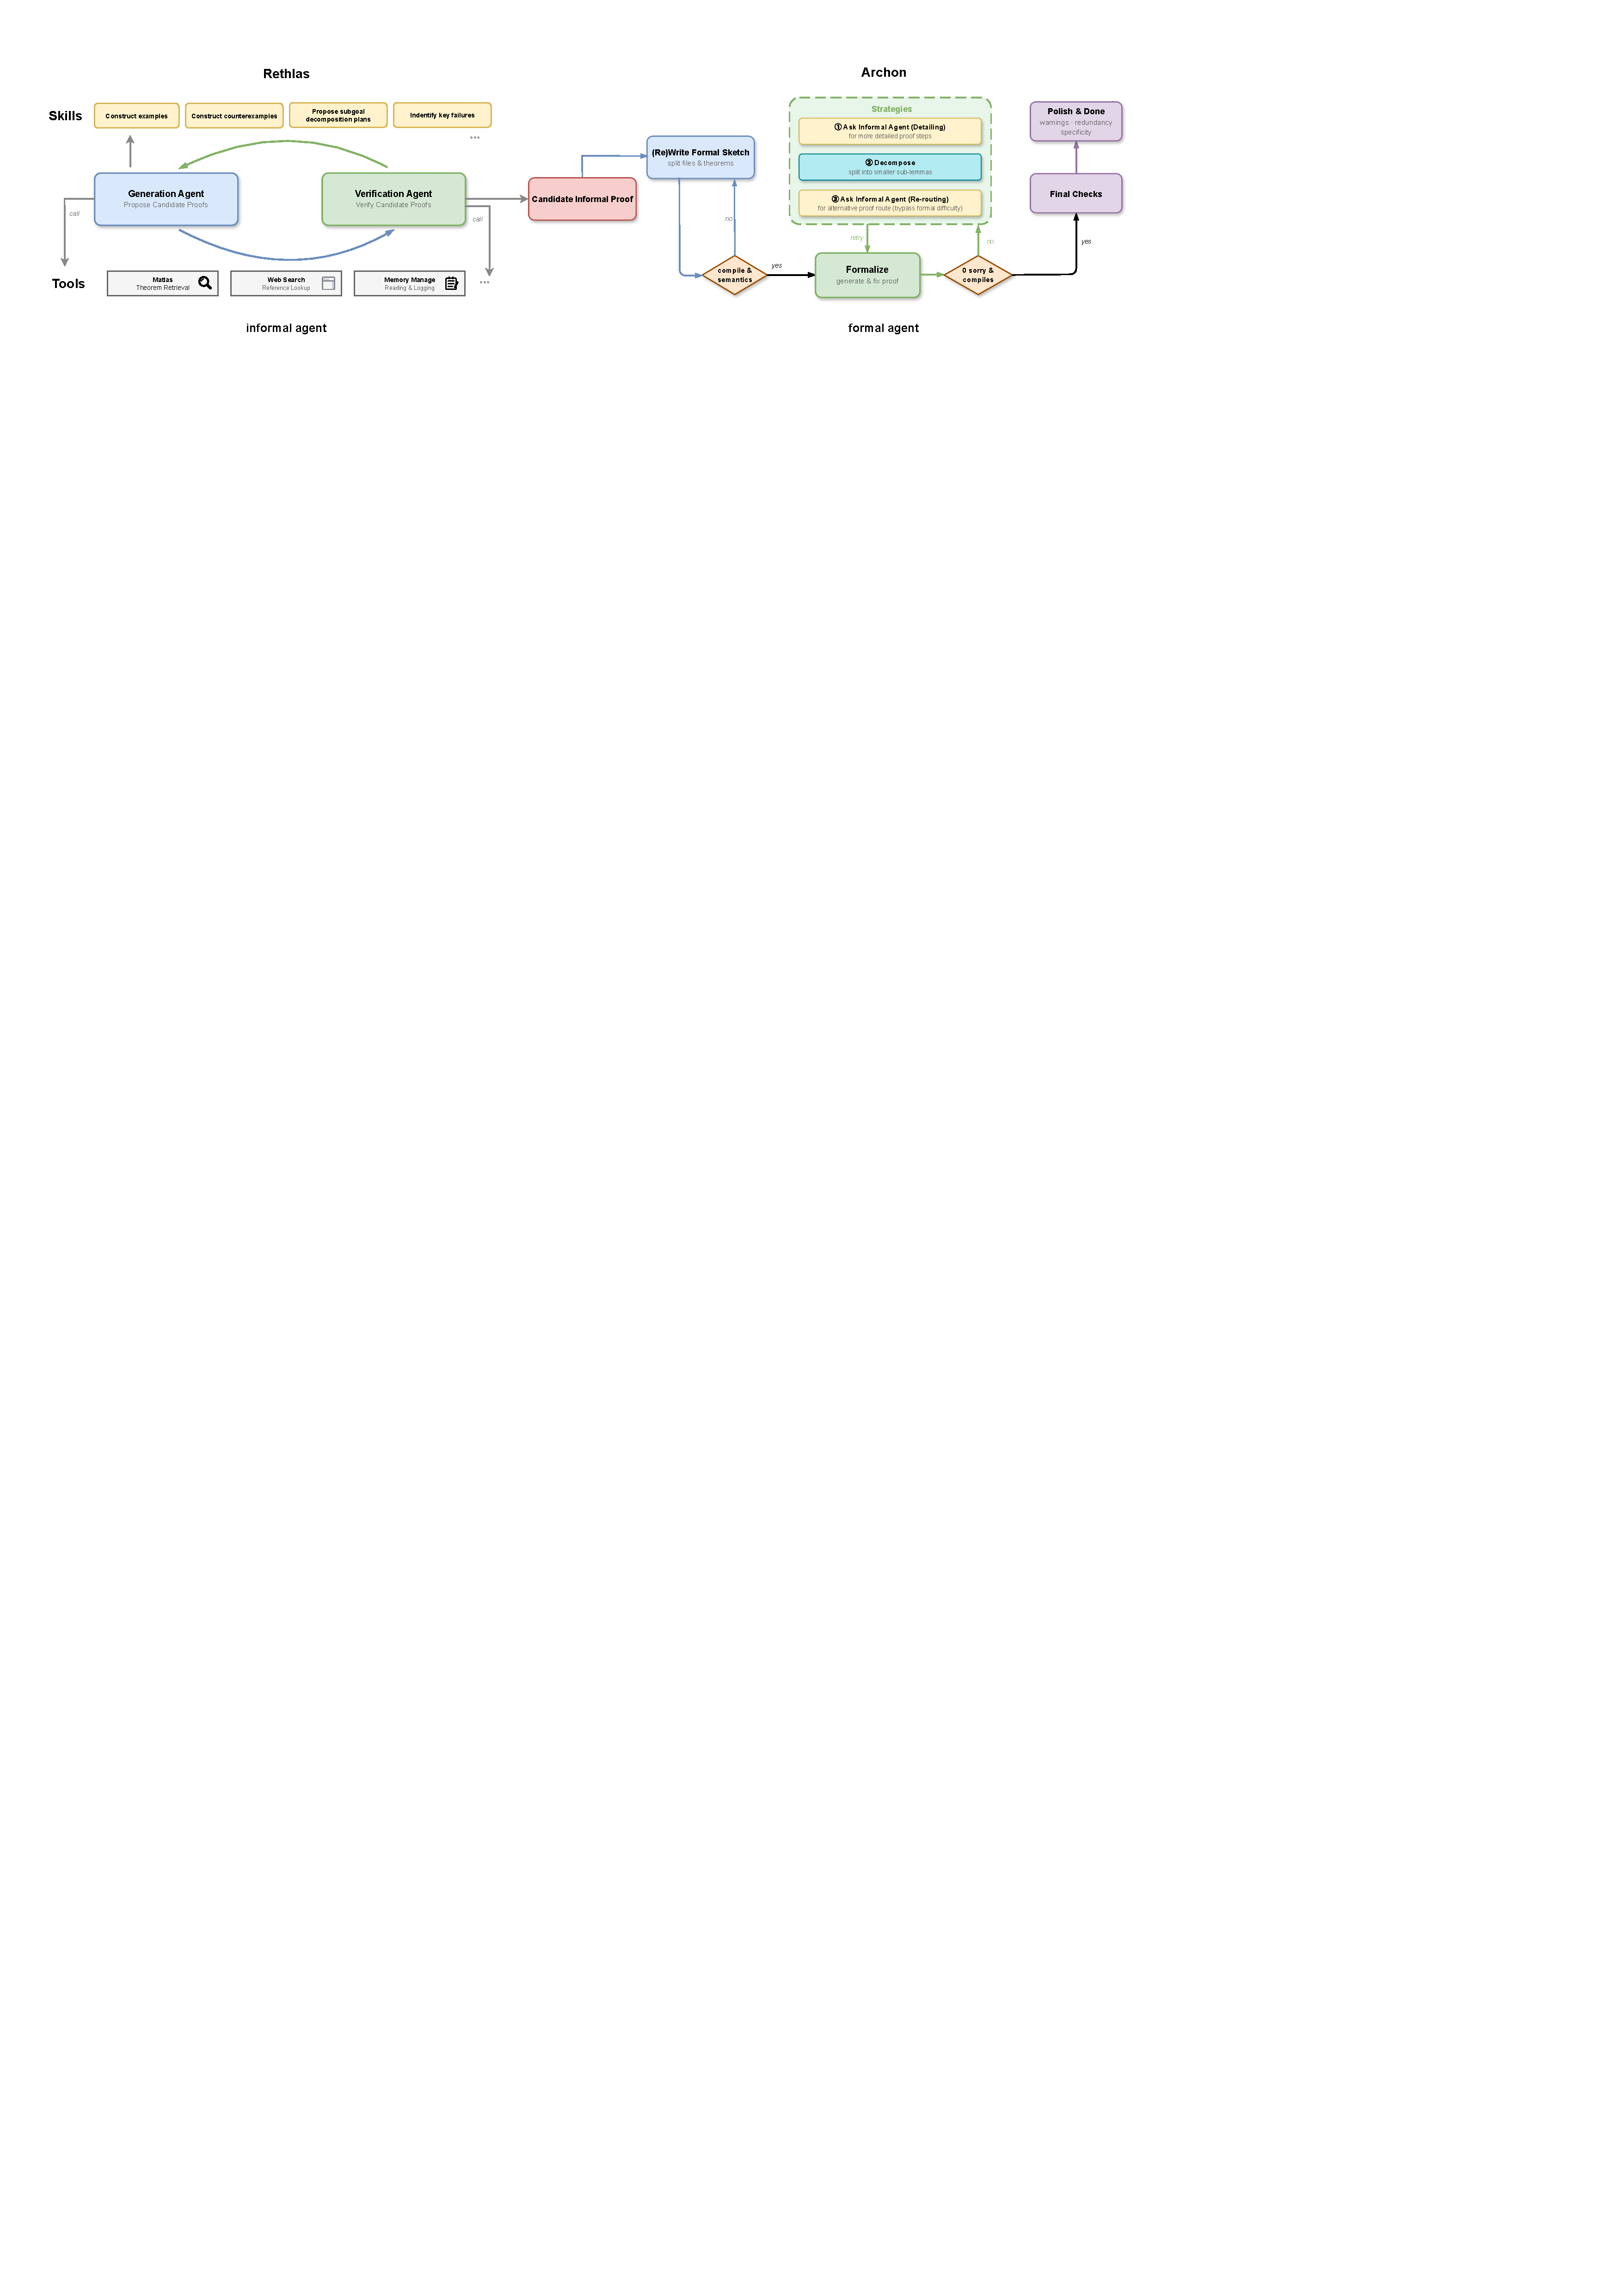
\includegraphics[width=0.99\linewidth]{figure/whole.pdf}
\caption{框架流程概述。}
\label{fig:complete}
\end{figure}




在本节中，我们描述了用于自主处理和验证研究级数学的框架。该框架包含一个非形式智能体（Rethlas），它首先生成一个潜在正确的候选证明，以及一个形式化智能体（Archon），它将这个非形式证明翻译成形式语言 Lean 4，并在形式化过程中填补任何空白（参见\Cref{fig:complete}）。非形式智能体 Rethlas 的设计呈现在\Cref{subsec:rethlas}中，而形式化智能体 Archon 的设计呈现在\Cref{subsec:archon}中。







\subsection{Rethlas：非形式智能体}\label{subsec:rethlas}








Rethlas 包含两个子智能体：生成智能体和验证智能体。如\Cref{fig:rethlas}所示，它在迭代过程中运行，其中生成智能体产生非形式证明并将其传递给验证智能体进行正确性检查。如果证明通过了验证，它被认为是一个候选非形式证明并且过程终止。否则，验证智能体会提供反馈，该反馈会传回生成智能体以修改证明。

\textbf{生成智能体。} 生成智能体旨在模仿人类数学家的工作流程，并配备了为数学研究量身定制的技能和工具。这些技能包含从数学家解决研究问题时采用的过程中提取的推理原语，它们包括：
\begin{itemize}
    \item \emph{构造玩具示例（toy examples）。} 当推理停滞不前并且需要更简单的实例来重新获得牵引力时使用此技能。构造的示例应该同时满足假设和结论，使人们能够观察假设如何生效并培养直觉。在应用此技能时，应该寻找示例中建议的重复模式、不变量或潜在的证明策略。推理、分解和检索也可用于识别合适的示例或简化设置。
    \item \emph{构造反例。} 当一个猜想或中间主张显得脆弱或不充分合理时使用此技能。目标是测试假设是否成立而结论失败。在应用此技能时，应利用推理、分解和检索来识别标准的障碍、病态构造或已知反例。
    \item \emph{搜索相关结果。} 此技能用于获取与当前问题相关的定理、构造、示例、反例或背景知识。它在构造示例或反例时，或者在证明需要支持性参考的子目标时也很有用。当发现可能有用的定理时，应使用来源的周围上下文展开所涉及的定义和概念，仔细验证其对当前设置的适用性，并明确不同上下文之间术语的任何变化。此外，不应仅停留在陈述本身，还应检查证明以提取有用的技术、构造、归约或证明模式。
    \item \emph{提出子目标分解计划。} 在从示例、反例、搜索结果和先前的尝试中收集到足够的见解后使用此技能。
    \item \emph{直接证明。} 一旦有一个或多个分解计划可用，就应用此技能。通过尝试直接证明其子目标来评估每个计划，同时在计划未完全成功时识别关键障碍。
    \item \emph{递归证明。} 当所有当前的分解计划都通过直接证明尝试过但没有一个完全成功时使用此技能。在这种情况下，会并行部署多个子智能体，每个子智能体分配一个分解计划以及与其相关的关键困难和其他计划中发现的困难。每个子智能体可以细化、扩展或局部修改其分配的计划，同时保持连续性而不是完全丢弃它。
    \item \emph{识别关键失败。} 当跨所有分解计划的递归尝试均失败时使用此技能。目标是识别这些失败中的常见模式，例如反复出现的障碍、无效的分解策略或缺失的背景知识。然后总结这些见解以指导下一轮计划生成。
\end{itemize}






\begin{figure}[tb]
\centering
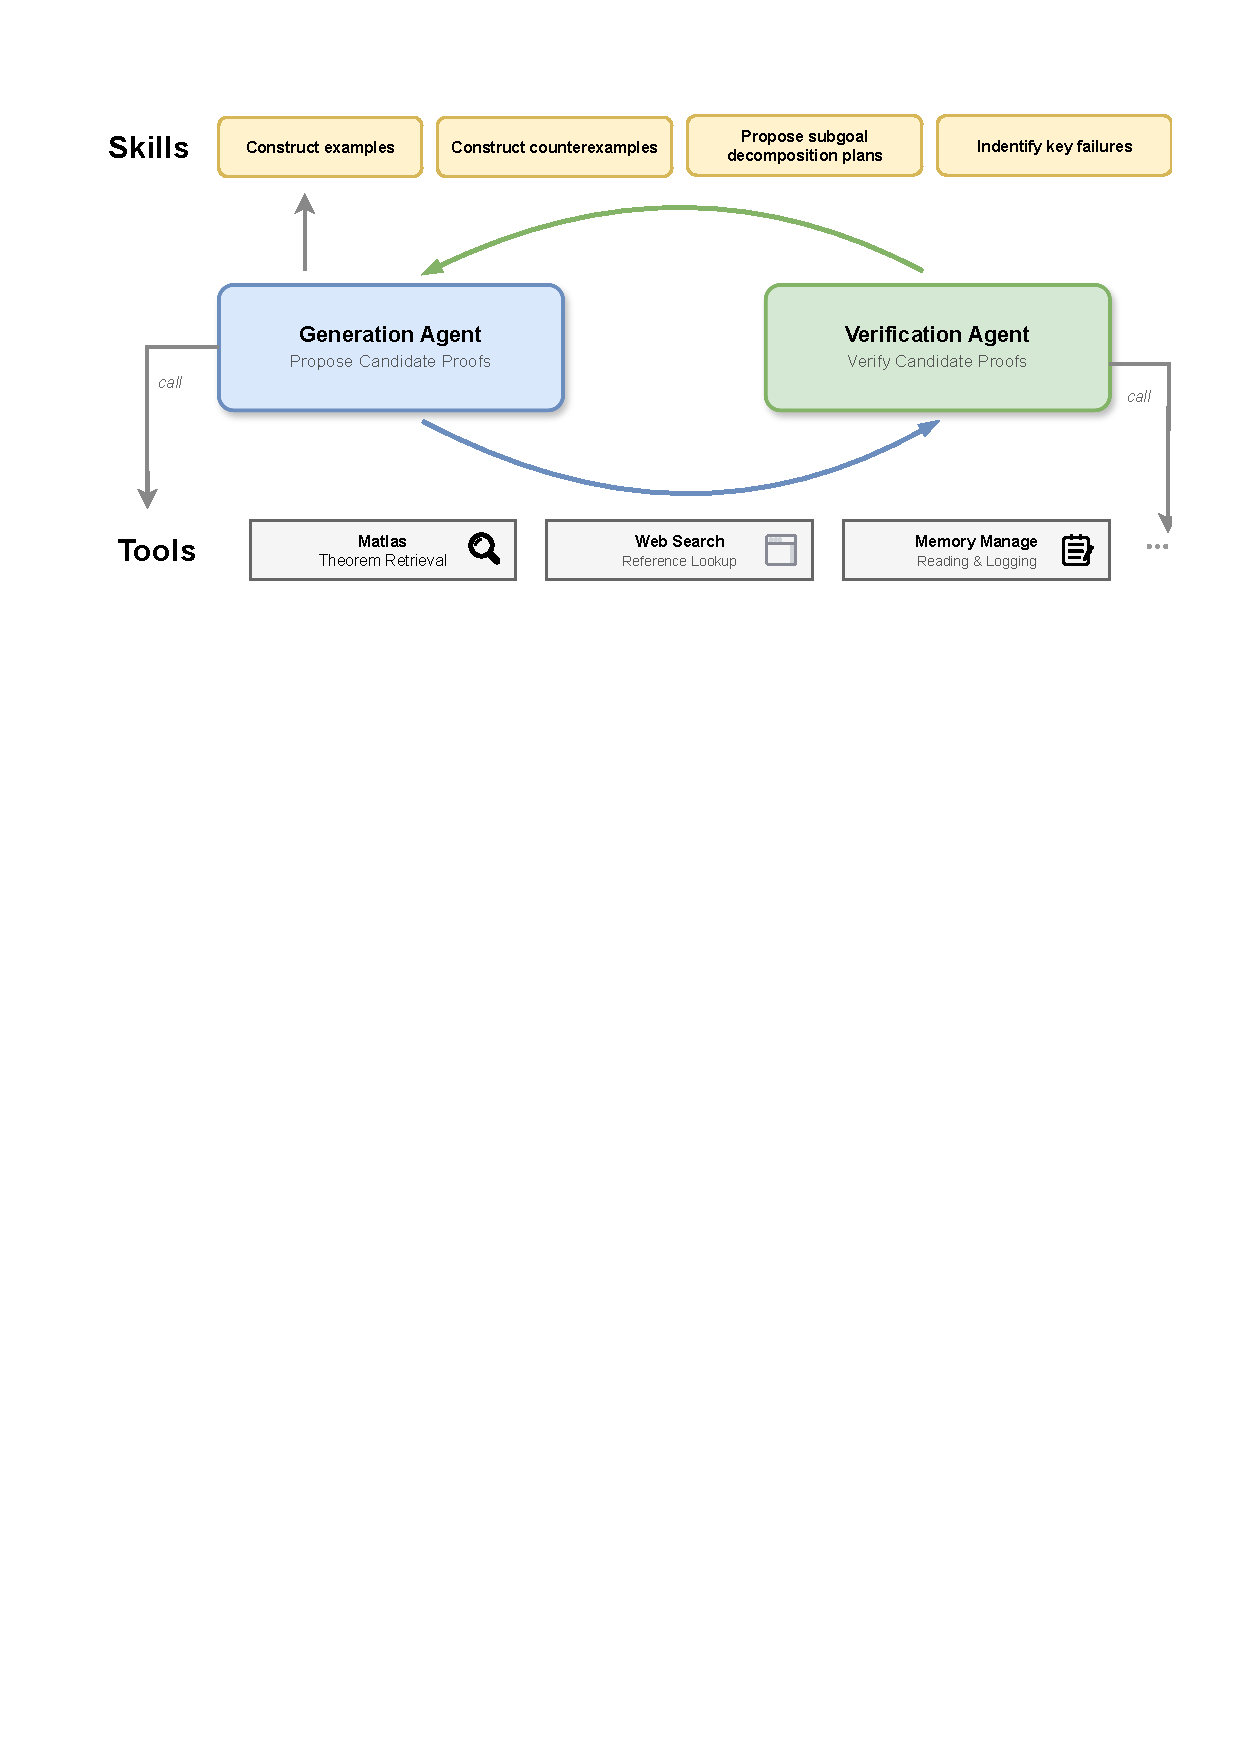
\includegraphics[width=0.6\linewidth]{figure/rethlas.pdf}
\caption{Rethlas 智能体。}
\label{fig:rethlas}
\end{figure}






正如上述描述所反映的那样，这些技能并不是孤立的，而是相互关联的。应用一项技能通常涉及其他技能的元素。例如，构造示例和反例并不是孤立发生的；它通常需要推理、问题分解和检索来识别适当的构造。在处理数学问题时，智能体被指示评估当前状态并选择要应用的适当技能，而不是事先决定固定的技能顺序。

在 Rethlas 使用的工具中，我们的定理搜索引擎 Matlas \footnote{Rethlas 实验中使用的 Matlas 版本是一个初步的内部测试系统，作为一个基于 arXiv 的定理搜索引擎，位于 \href{https://leansearch.net/thm/}{https://leansearch.net/thm/}。其语料库包含大约 1360 万条直接从 arXiv 论文中提取而未进一步处理的数学陈述。我们最新的 Matlas 系统，位于 \href{https://matlas.ai/}{https://matlas.ai/}，是一个更高级的定理搜索引擎，建立在从 180 种期刊和 1900 多本教科书的 435K 篇已发表论文中收集的 851 万条陈述之上。因此，它提供了更可靠和精选的数学结果来源。此外，我们提取陈述依赖关系并执行层次展开以使陈述更加自包含，这与早期基于 arXiv 的版本相比进一步提高了它们的可用性和质量。之前基于 arXiv 的定理搜索引擎将在不久的将来被弃用。} 发挥着核心作用。在我们的实验中，Matlas 作为一个针对 arXiv 数学陈述（包括定义、命题、定理、推论、示例和注记）的语义搜索引擎。其语料库包含大约 1360 万条这样的陈述，每条都嵌入到一个向量数据库中。给定一个数学陈述形式的查询，Matlas 嵌入查询并使用余弦相似度执行最近邻搜索以检索相关结果。与一般网络搜索相比，Matlas 提供了一种更细粒度且有原则的针对数学内容的检索机制。虽然其语料库较小，但它更加结构化，并能够更精确地识别相关陈述。在应用 \texttt{search-math-results} 技能时，Rethlas 被指示首先查询 Matlas 并检索相关的定理、示例或反例。然后它可以随后使用网络搜索要么跟进并查找原始论文进行详细检查，要么在 Matlas 结果不够用时补充搜索结果。

此外，Rethlas 维护一个工作内存，记录在推理过程中生成的中间工件，例如构造的示例、反例和子目标分解计划。智能体被指示将这些工件写入内存，并在需要时查询此内存，从而实现对先前生成见解的重用，并提高跨推理步骤的连贯性。在我们的实验中，生成智能体是使用 OpenAI Codex 智能体框架实现的，以 GPT-5.4 作为基础模型。

\textbf{验证智能体。} 验证智能体配备了检查数学证明正确性的技能。这些包括顺序验证陈述，例如检查跳过或含糊的步骤，识别关键错误和漏洞，以及仔细评估表面上未使用的假设是否真的多余，或者相反表明论证有遗漏。它们还包括确认引用的陈述，通过使用我们的定理搜索工具 Matlas 和网络搜索，检查被引用的陈述是否存在且适用于当前上下文，使用源论文的上下文扩展引用的陈述中的定义和术语，并确保当前证明中使用的术语与被引用来源中的术语具有相同的含义，因为相同的词语在不同的上下文中可能具有不同的定义。在我们的实验中，验证智能体是使用 OpenAI Codex 智能体以 GPT-5.4 作为底层模型实现的。

